\chapter{Lecture 15: Properties of Analytic Functions}

\section{Maximum Modulus \& Mean Value}

\begin{theorem}
    [The Open Mapping Theorem]
    if $f$ is analytic on a Domain $D$, then either:
    \begin{itemize}
        \item $f$ is constant
        \item $f(D) \subseteq D$ is open
    \end{itemize}
\end{theorem}

\begin{proof}
    Recall that if $\Re(f) =  0$, then $f$ is constant
    Suppose $f$ is analytic, but not constant.\\
    Let $w_0 = f(z_0)$\\
    Since $f$ is not constant, we choose $r > 0$ (small), such that $f(z) - w_0$ has no zero in the set of $0 < |z -z_0| < r$\\
    \textbf{\underline{Why?}: Since zeroes of analytic functions are isolated}

    Let $0 < \delta = \min_{z \in |z - z_0|  = r} |f (z) - w_0| > 0$\\
    if $|w - w_0| < \delta$, then on $|z - z_0|  = r$:
    \begin{align*}
        |(f (z) - w) - (f(z) - w_0)| = |w- w_0| < \delta \leq |f(z) - w_0|
    \end{align*}
    By Rouche's Theorem, $f(z) - w$ has the same number of zeroes in $|z - z_0| \leq r$ as $f(z) - w_0$  (in particular, at least 1)
    \begin{align*}
        \Rightarrow w \in f(D) \text{ so } & \forall w \,| \,|w - w_0| < \delta, \exists z \in D \, | \, f(z)  = w \\
                                           & \{|w - w_0| < \delta  \in f(D)\}
    \end{align*}
    So $f(D)$ is open
\end{proof}

\begin{definition}
    [Mapping]
    A function $f: D \to \mathbb{C}$ is said to be $m \to 1$ at $z_0 \in D$ if in the neighborhood around $z_0$ there are exactly $m$ points in the domain $z$ that map to the same point $w = f(z_0)$ in the codomain.
\end{definition}

\begin{corollary}

    if $f$ is a non-constant analytic function on $D$ and $f(z) - f(z_0)$ has a zero of order $m$ at $z_0$, then $f(z)$ is $m \to 1$ map near $z_0$, in particular, if $f'(z_0) = 0$, then $f$ is not $1 \to 1$ in any disc around $z_0$. Furthermore, any disc around $z_0$ contains $m$ points $z \neq z_0$ such that $f(z) = f(z_0)$
\end{corollary}

\begin{example}
    if $f(z) = z^2$, has a zero of order $2$ at $0$\\
    if $z \neq 0$, then $f(z) = f(-z)$, so $f$ is $2 \to 1$
\end{example}
\begin{figure}[H]
    \centering
    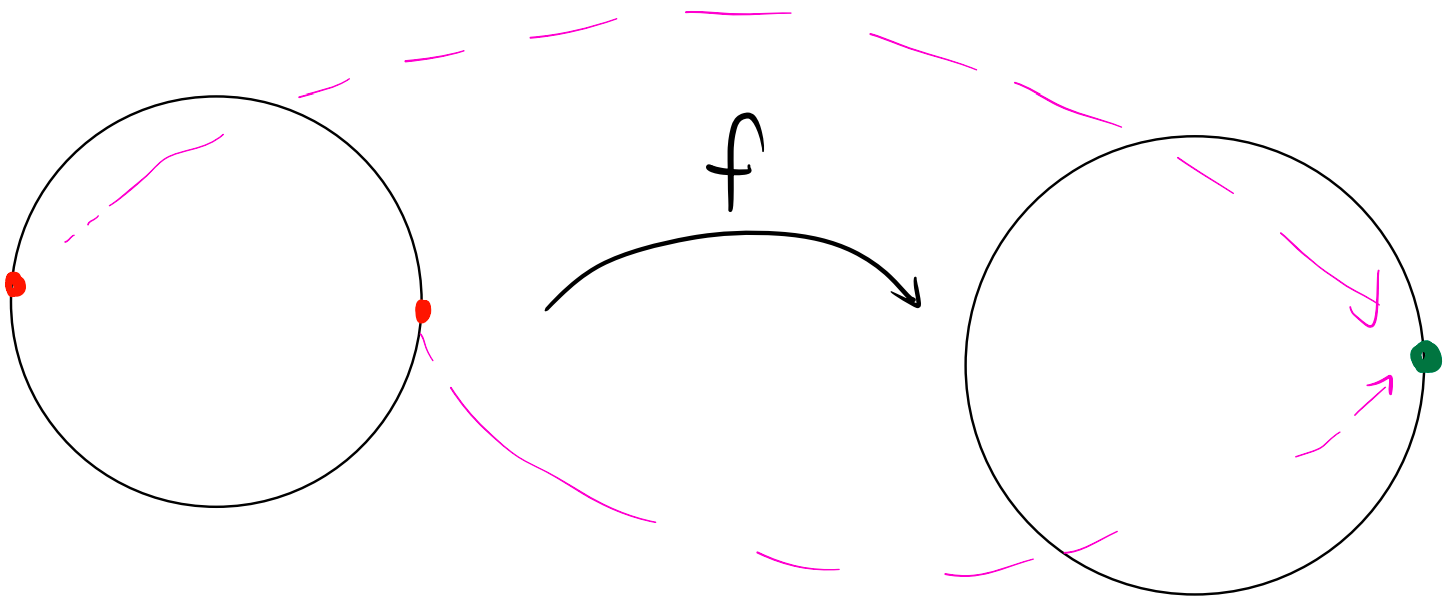
\includegraphics[width=0.5\textwidth]{LECTURE_15/max-mod.png}
    \caption{Mapping of $f(z) = z^2$}
\end{figure}
\begin{corollary}
    [Maximum Modulus Principle]
    if $f$ is a non-constant analytic function on the domain $D$, then $|f|$ has no local maximum.
\end{corollary}

\begin{remark}
    This may seem counterintuitive, but this is unique to complex functions. It is possible for a real differentiable function, $f$, to be non-constant and $|f|$ to have a local maximum.
\end{remark}

\begin{proof}
    Suppose $|f|$ has a local max at $z_0$, i.e.:
    $$|f(z)| \leq |f(z_0)| \quad \forall |z - z_0| \leq r$$
    For some $r > 0$, then $f(z_0)$ lies on the boundary of the set $\{f(z) \, | \, |z - z_0| < r\}$ because the maximum modulus in an open set is on the boundary, which is a contradiction to the open mapping theorem which states that $f(D)$ is open.
\end{proof}

\begin{theorem}
    [Schwartz Lemma]
    Suppose $f$ is analytic in a disc:
    \begin{align}
        \{|z| < 1\}, f(0) = 0 \text{ and } |f(z)| \leq 1 \forall |z| < 1 \\
    \end{align}
    \underline{Then} $|f(z)| \leq |z|\, \forall \, |z| < 1$, \underline{and}
    \begin{align}
        |f(\tilde{z})| & = |\tilde{z}| \text{ for some } z \neq 0, \text{ if and only if} \\
        f(z)           & = \lambda z \text{ for } \lambda \in \mathbb{C}, |\lambda| = 1
    \end{align}
\end{theorem}

\begin{proof}
    Say:
    \begin{align*}
        g(z) = \frac{f(z)}{z}, \quad |z| < 1
    \end{align*}
    Since $f(0) = 0$ we know $g(z) = \frac{f(z)}{z}$ is analytic for $|z| < 1$\\
    And on $|z| = r \quad (r < 1)$ we can write:
    \begin{align}
        |g(z)| \leq \frac{|f(z)|}{r} \leq \frac{1}{r}
    \end{align}
    So, by max modulus principle:
    \begin{align*}
        |g(z)| & < \frac{1}r \text{ on } \{|z| \leq r\} \\
    \end{align*}
    Because $\{g(z) \, : \, |z| = r \to 1\}$ needs to be open.\\
    Taking $r \to 1$, conclude
    \begin{align*}
        |g(z)| \leq \frac{|f(z)|}{|z|} \leq 1 \to f(z) \leq |z|
    \end{align*}
    We say $f(z) \leq |z|$ because $z \leq 1$, so we don't worry about openness.\\
    if $|f(z_0)| = |z_0|$, for some\\
    \textbf{Then} $|g(z)| = 1$, so $g(z)$ has an interior maximum. This means $g(z)$ is constant, so $f(z) = \lambda z$ for $|\lambda| = 1$
\end{proof}

\section{Mean-Value Property}
\begin{theorem}
    Suppose \( f = u + iv \) is analytic on \( \{ |z - z_0| \leq r \} \). Then, for any \( s \leq r \),

    the average value of \( u \) and \( v \) on the circle \( |z - z_0| = s \) is given by:
    \[
        \begin{rcases}
            u(z_0) = \frac{1}{2\pi} \int_{0}^{2\pi} u(z_0 + se^{i\theta}) \, d\theta \\
            v(z_0) = \frac{1}{2\pi} \int_{0}^{2\pi} v(z_0 + se^{i\theta}) \, d\theta
        \end{rcases} = \text{Average value of } u \text{ or } v \text{ on the circle } |z - z_0| = s
    \]
\end{theorem}


\begin{proof}
    \textbf{Cauchy's Integral Formula} with $\gamma(\theta) = z_0 + se^{i\theta}$:
    \begin{align*}
        f(z_0)                                      & = \frac{1}{2\pi i} \int_{|z - z_0| = s} \frac{f(z)}{z - z_0}dz                                    \\
        \rightarrow z = z_0 + se^{i\theta} \quad dz & = ise^{i\theta}d\theta                                                                            \\
        f(z_0)                                      & = \frac{1}{2\pi i} \int_{0}^{2\pi} \frac{f(z_0 + se^{i\theta})}{se^{i\theta}}ise^{i\theta}d\theta \\
    \end{align*}
    Now we take the real and imaginary parts of the above equation to get the average value of \( u \) and \( v \) on the circle \( |z - z_0| = s \).

\end{proof}

\section{Fractional Linear Transformations}

\begin{definition}
    [Fractional Linear Transformation]
    A FLT is a rational function of the form:
    \begin{align*}
        T(z) = \frac{az + b}{cz + d} \quad a,b,c,d \in \mathbb{C}, ad - bc \neq 0
    \end{align*}
\end{definition}

\begin{remark}
    Note: if $ad = bc$, then:
    \begin{align*}
        T'(z) = \frac{a (cz + d) - (az + b)c}{(cz + d)^2} = \frac{ad - bc}{(cz + d)^2} = 0
    \end{align*}
    So $T(z)$ is constant, and we're not interested in constant functions
\end{remark}

\begin{claim}
    $T$ is $1 \to 1$\\
    If $T(z_1) = T(z_2) \implies z_1 = z_2$.
    \begin{proof}
        \begin{align*}
            \frac{az_1 + b}{cz_1 + d}         & = \frac{az_2 + b}{cz_2 + d}    \\
            \iff acz_1^2 + adz_1 + bcz_1 + bd & = acz_2^2 + adz_2 + bcz_2 + bd \\
            (ad - bc)z_1                      & = (ad - bc)z_2                 \\
            z_1                               & = z_2
        \end{align*}
    \end{proof}
\end{claim}

\begin{claim}
    [T has an inverse]
    \begin{align*}
        T^{-1}(z) = \frac{dz - b}{-cz + a}
    \end{align*}
    Which is also a FLT
    \begin{proof}
        \begin{align*}
            T(z)                  & = w                          \\
                                  & = \frac{az + b}{cz + d}      \\
            \rightarrow z         & = \frac{dw - b}{-cw + a}     \\
            \rightarrow T^{-1}(w) & = \frac{dw - b}{-cw + a} = z
        \end{align*}
    \end{proof}
\end{claim}

\begin{claim}
    [Composition of FLT]
    if $T_1, T_2$ are FLT, then $T_1 \circ T_2$ is also a FLT
    \begin{proof}
        \begin{align*}
            T_1(z)      & = \frac{a_1z + b_1}{c_1z + d_1}                                                             \\
            T_2(z)      & = \frac{a_2z + b_2}{c_2z + d_2}                                                             \\
            T_1(T_2(z)) & = \frac{a_1(\frac{a_2z + b_2}{c_2z + d_2}) + b_1}{c_1(\frac{a_2z + b_2}{c_2z + d_2}) + d_1} \\
                        & = \frac{(a_1a_2z + a_1b_2 + b_1c_2z + b_1d_2)}{(c_1a_2z + c_1b_2 + d_1c_2z + d_1d_2)}       \\
                        & = \frac{(a_1a_2z + b_1b_2)}{(c_1a_2z + d_1b_2)}                                             \\
                        & = \frac{a_1a_2z + b_1b_2}{c_1a_2z + d_1b_2}                                                 \\
        \end{align*}
    \end{proof}
\end{claim}

\subsection{Matrix Representation of FLT}

\begin{theorem}
    Given $T(z) = \frac{az + b}{cz + d}$, we can represent $T$ as a matrix:
    $$A_T = \begin{pmatrix}
            a & b \\
            c & d
        \end{pmatrix}$$
    Where $A_T$ is a $2 \times 2$ matrix with determinant $ad - bc \neq 0$. So, $A_T$ is invertible
\end{theorem}

\begin{remark}
    Also:
    \begin{align*}
        A_{T_1 \circ T_2} = A_{T_1}A_{T_2}
    \end{align*}
    Note: if $\lambda \in \mathbb{C}, \lambda \neq 0$, then $A$ and $\lambda A$ give rise to the same FLT.
\end{remark}

\subsection{Point at Infinity}
\begin{definition}
    Recall that we can add the point at $\infty$ to $\mathbb{C}$ to get the $2$ sphere $S^2 = \mathbb{C} \cup \{\infty\}, \{x^2 + y^2 + z^2 = 1\}$
\end{definition}

\begin{figure}[H]
    \centering
    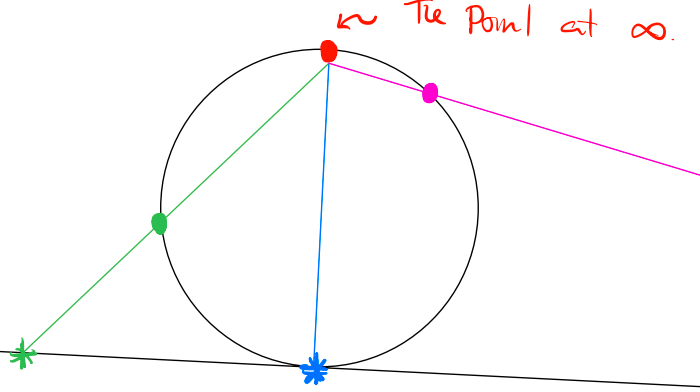
\includegraphics[width=0.5\textwidth]{LECTURE_15/s2.png}
    \caption{The Riemann Sphere}
\end{figure}

\begin{remark}
    An FLT should be be thought of in terms of how it moves points in $S^2$
\end{remark}

\begin{theorem}
    Consider $T(z) = \frac{a z + b}{c z + d}, (c \neq 0)$
    \begin{itemize}
        \item when $z = \frac{-d}{c}$, $T(z) = \infty$
        \item $\lim_{z \to \infty} T(z) = \frac{a + \frac{b}{z}}{c + \frac{d}{z}} = \frac{a}{c}$
    \end{itemize}
\end{theorem}

\begin{example}
    If $a, c = 1$, Then ($d \neq 0$):
    \begin{itemize}
        \item $T(0) = \frac{b}{d}$
        \item $T(\infty) = \frac{1}{d}$
        \item $T(\frac{-d}{c}) = \infty$
    \end{itemize}
\end{example}

\subsection{Fixed Points}

\begin{definition}
    [Fixed Points]
    A fixed point of $T(z) = z$ is a point $z_0$ such that $T(z_0) = z_0$
\end{definition}

\begin{lemma}
    An FLT has either $\leq 2$ fixed points or $\infty$ fixed points (it's the identity function)
\end{lemma}
\begin{proof}
    \begin{align*}
        T(z) & = \frac{az + b}{cz + d} = z \\
    \end{align*}
    So:
    \begin{align*}
        cz^2 + (d - a)z - b & = 0
    \end{align*}
    So, $z$ has at most $2$ solutions, unless $c = 0$, in which case $T(z) = z$ for all $z$
\end{proof}

\begin{proposition}
    A consequence of the above lemma is that if we're given:
    \begin{align*}
        \{z_1, z_2, z_3\} & \ \mathbb{C} \cup \{\infty\} = S^2  \quad \text{distinct}                  \\
                          & \{w_1, w_2, w_3\} \subset \mathbb{C} \cup \{\infty\} \quad \text{distinct} \\
    \end{align*}
    Then, there exists a unique FLT $T$ such that $T(z_i) = w_i,\quad i = 1, 2, 3$
\end{proposition}
\begin{proof}
    Consider:
    \begin{align*}
        L(z) = \frac{z - z_1}{z - z_3} \cdot \frac{z_2 - z_3}{z_2 - z_1}
    \end{align*}
    Then:
    \begin{itemize}
        \item $L(z_1) = 0$
        \item $L(z_2) = 1$
        \item $L(z_3) = \infty$
    \end{itemize}
    \textbf{Similarly}
    \begin{align*}
        S(w) = \frac{w - w_1}{w - w_3} \cdot \frac{w_2 - w_3}{w_2 - w_1}
    \end{align*}
    Then:
    \begin{itemize}
        \item $S(w_1) = 0$
        \item $S(w_2) = 1$
        \item $S(w_3) = \infty$
    \end{itemize}
    So, $S^{-1} \circ L$ is the FLT we're looking for. $T$ is unique since if $\tilde{T}$ maps $z_1 \to w_1$, then $T^{-1} \circ \tilde{T} (f)$ fixes $z_1, z_2, z_3$, so it must be the identity function.
    \begin{align*}
        \tilde{T} = T
    \end{align*}
\end{proof}